\documentclass[a4paper]{scrartcl}
\usepackage{amsmath,amssymb,graphicx,amsthm, amssymb, amsfonts}
\usepackage[utf8]{inputenc}
\usepackage[english]{babel}

\usepackage[x11names,svgnames,dvipsnames]{xcolor}

\usepackage{float}
\usepackage{multicol}  
%\usepackage[rflt]{floatflt}  
\usepackage{graphics}
\usepackage{epsfig} 
%\usepackage{qtree} 
\usepackage{textcomp}
\usepackage{url}

% PDF Import support
\usepackage{pdfpages}
% Support for PDF scaling
\usepackage{graphicx}
% Algorithmen
\usepackage{algorithmic}
\usepackage{algorithm}
\usepackage{listings} 
% \lstset{numbers=left, numberstyle=\tiny, numbersep=5pt} 
\lstset{
	basicstyle=\ttfamily\scriptsize\mdseries,
	keywordstyle=\bfseries\color{blue},
	identifierstyle=,
% 	stringstyle=\itshape\color{red},
	numbers=left,
	numberstyle=\tiny,
	stepnumber=10,
	breaklines=true,
	frame=none,
	showstringspaces=false,
	tabsize=4,
% 	backgroundcolor=\color{gray},
% 	morecomment=[s][\color{green}]{/+}{+/},
	commentstyle=\color{gray},	
	captionpos=b,
	float=htbp,
}
\newcommand{\norm}[1]		{\left|\left| #1 \right|\right|}
\newcommand{\mbf}[1]		{\mathbf{#1}}

\newcommand{\K}     {\mathbb{K}}

%%% Nice Blockquote from 
%% http://tex.stackexchange.com/questions/16964/block-quote-with-big-quotation-marks
% \usepackage[svgnames]{xcolor}

  \usepackage[utf8]{inputenc}
  \usepackage[T1]{fontenc}
  \usepackage{libertine} % or any other font package (or none)
  \newcommand*\quotefont{\fontfamily{fxl}} % selects Libertine for quote font
\usepackage{tikz}
\usepackage{framed}
% Make commands for the quotes
\newcommand*{\openquote}{\tikz[remember picture,overlay,xshift=-15pt,yshift=-12pt]
     \node (OQ) {\quotefont\fontsize{60}{60}\selectfont``};\kern0pt}
\newcommand*{\closequote}{\tikz[remember picture,overlay,xshift=15pt,yshift=10pt]
     \node (CQ) {\quotefont\fontsize{60}{60}\selectfont''};}
% select a colour for the shading
\definecolor{shadecolor}{named}{LightGoldenrodYellow}
% wrap everything in its own environment
\newenvironment{shadequote}%
{\begin{snugshade}\begin{quote}\openquote}
{\hfill\closequote\end{quote}\end{snugshade}}
%% End Blockquote

\newcommand\novspace{\@minipagetrue}
\newtheorem*{definition}{Definition}

\let\oldemph\emph
\renewcommand{\emph}[1]{{\color{DeepSkyBlue4}{\oldemph{#1}}}}


\author{Pascal Spörri\\pascal@spoerri.io}
\title{Concepts of Object Oriented Programming\\Summary HS 2012}
%\thanks{Licence: Creative Commons Attribution-Share Alike 3.0 Unported (\url{http://creativecommons.org/licenses/by-sa/3.0/})}}
\date{\today}
\usepackage[colorlinks=false,pdfborder = {0 0 0 0}]{hyperref}


\begin{document}
\maketitle
\newpage
\part{Introduction}
\section{Requirements}
With time programming languages received more and more requirements.
\begin{figure}[h!]
  \centering
    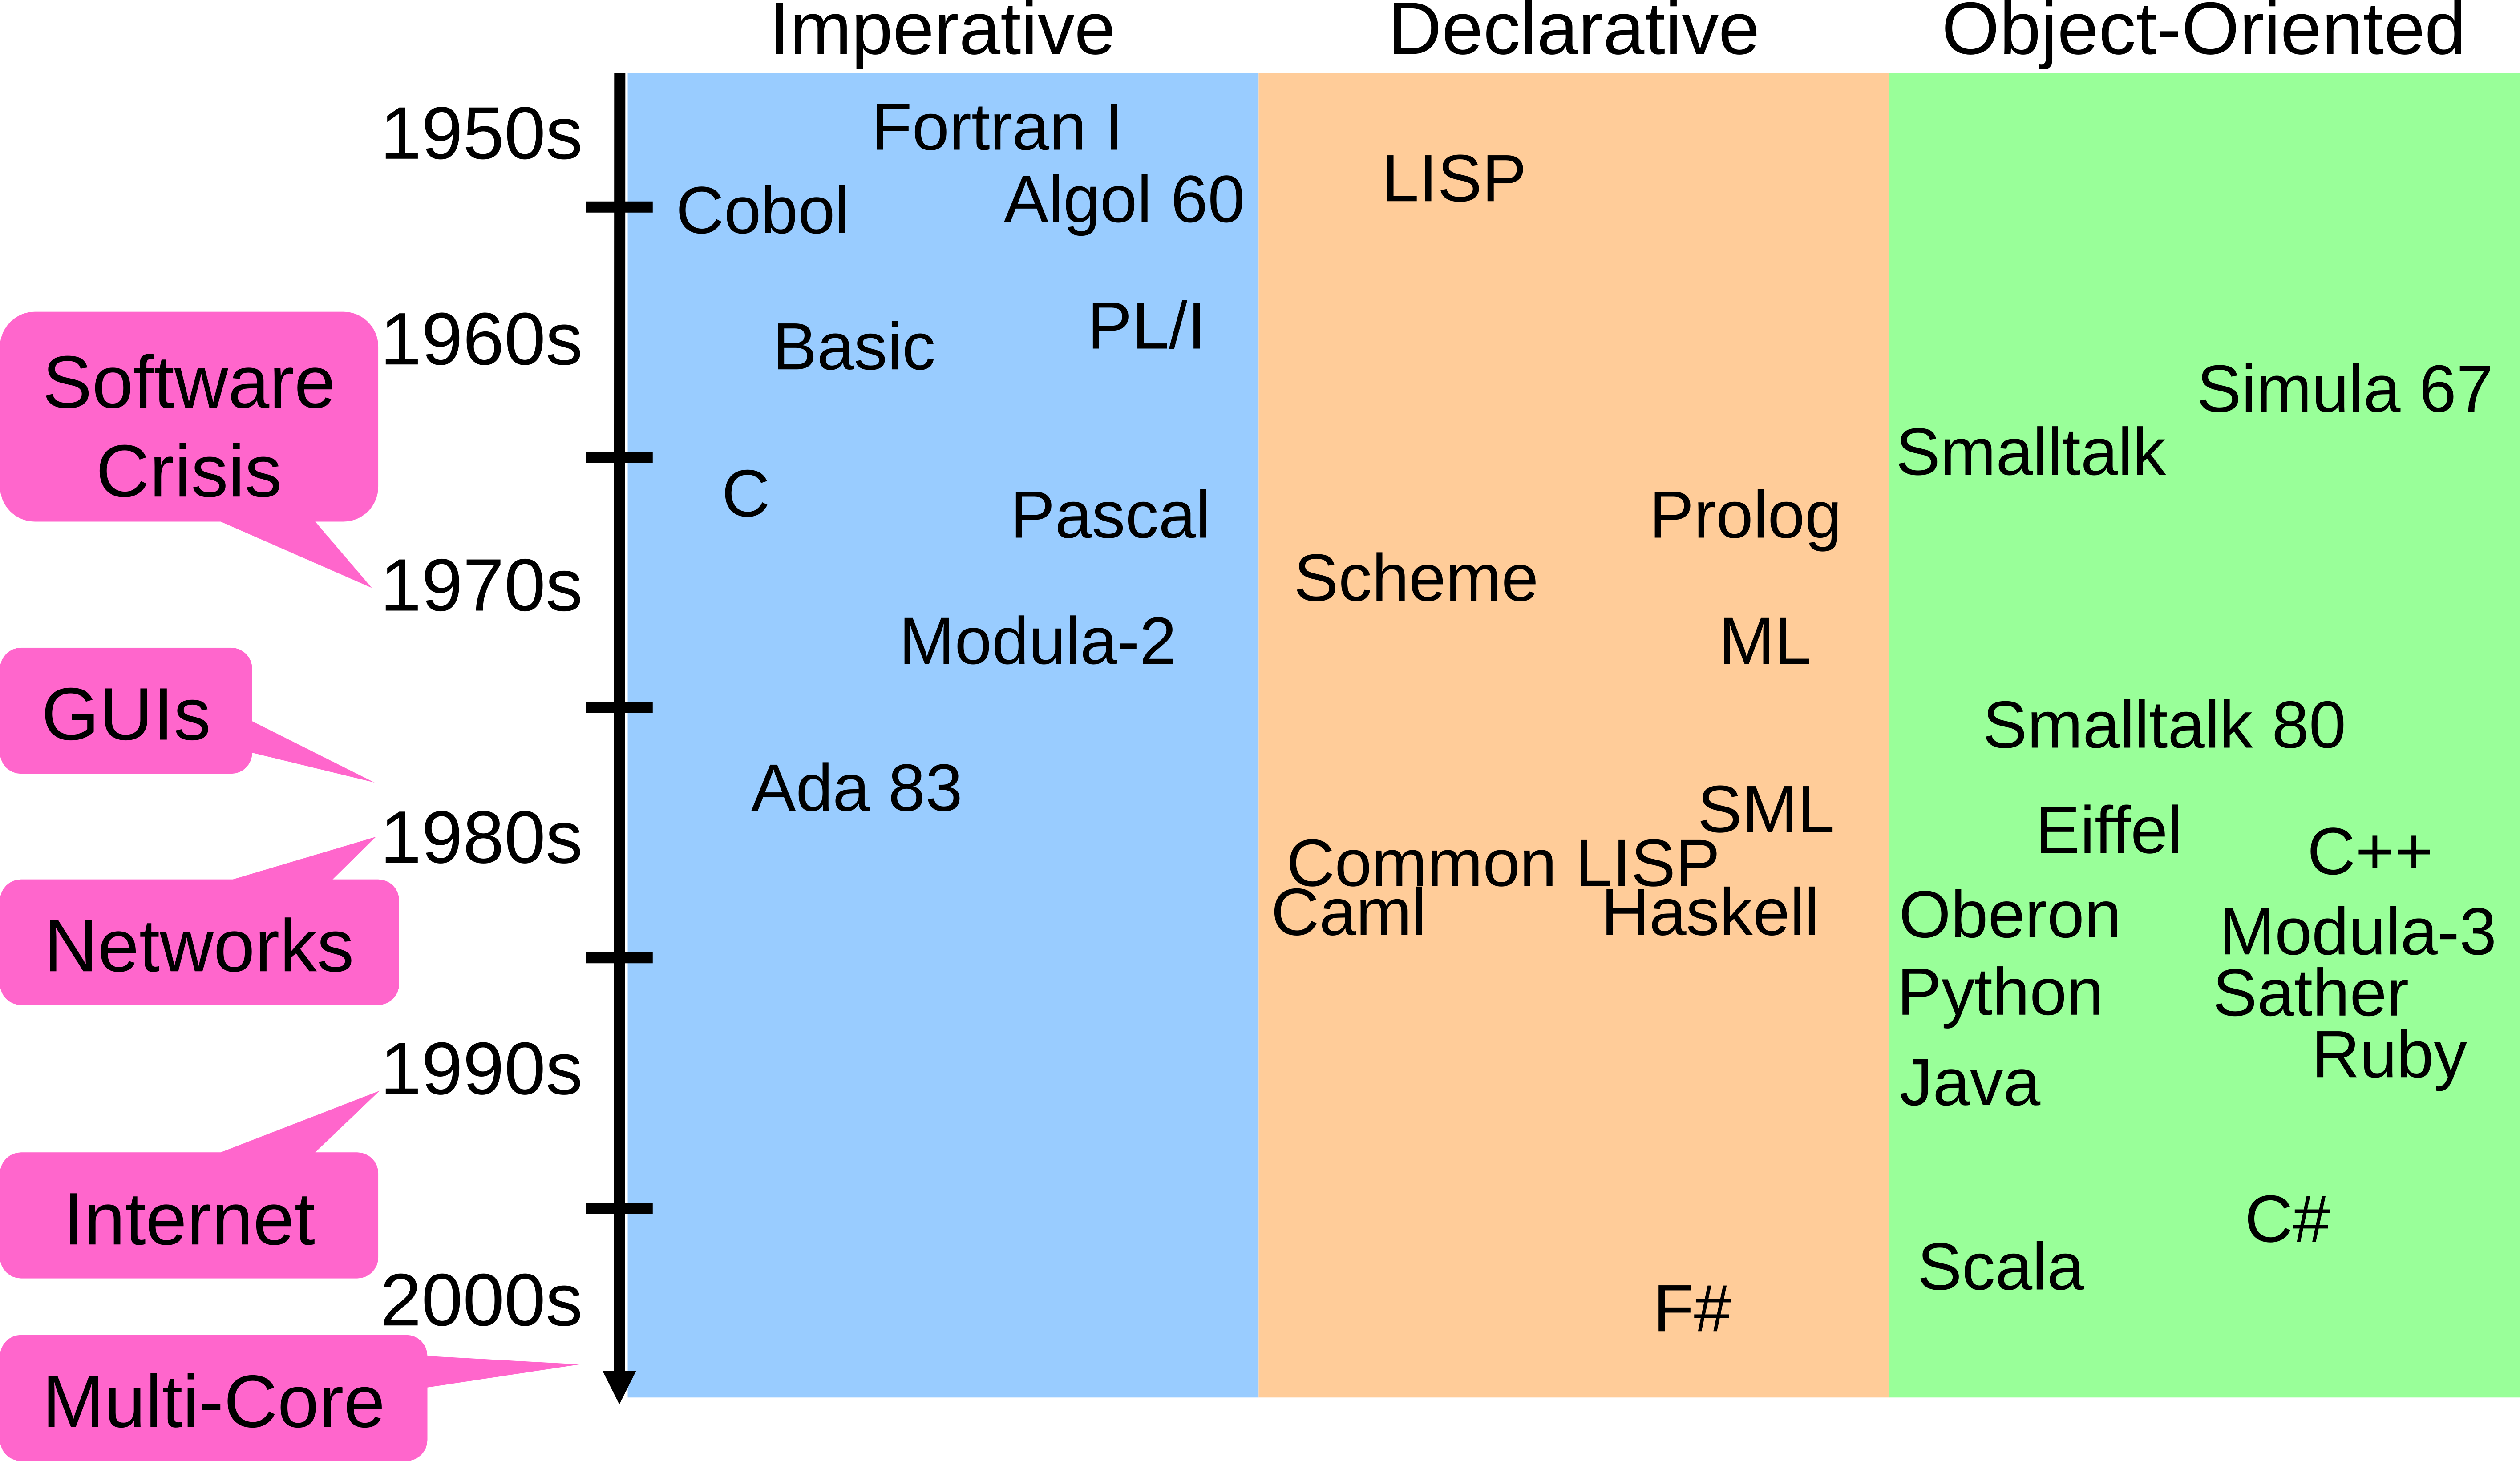
\includegraphics[width=0.7\textwidth]{img/01_programming_languages}
      \caption{History of Programming Languages}

\end{figure}

Which forced a rethinking process.
\begin{figure}[h!]
  \centering
    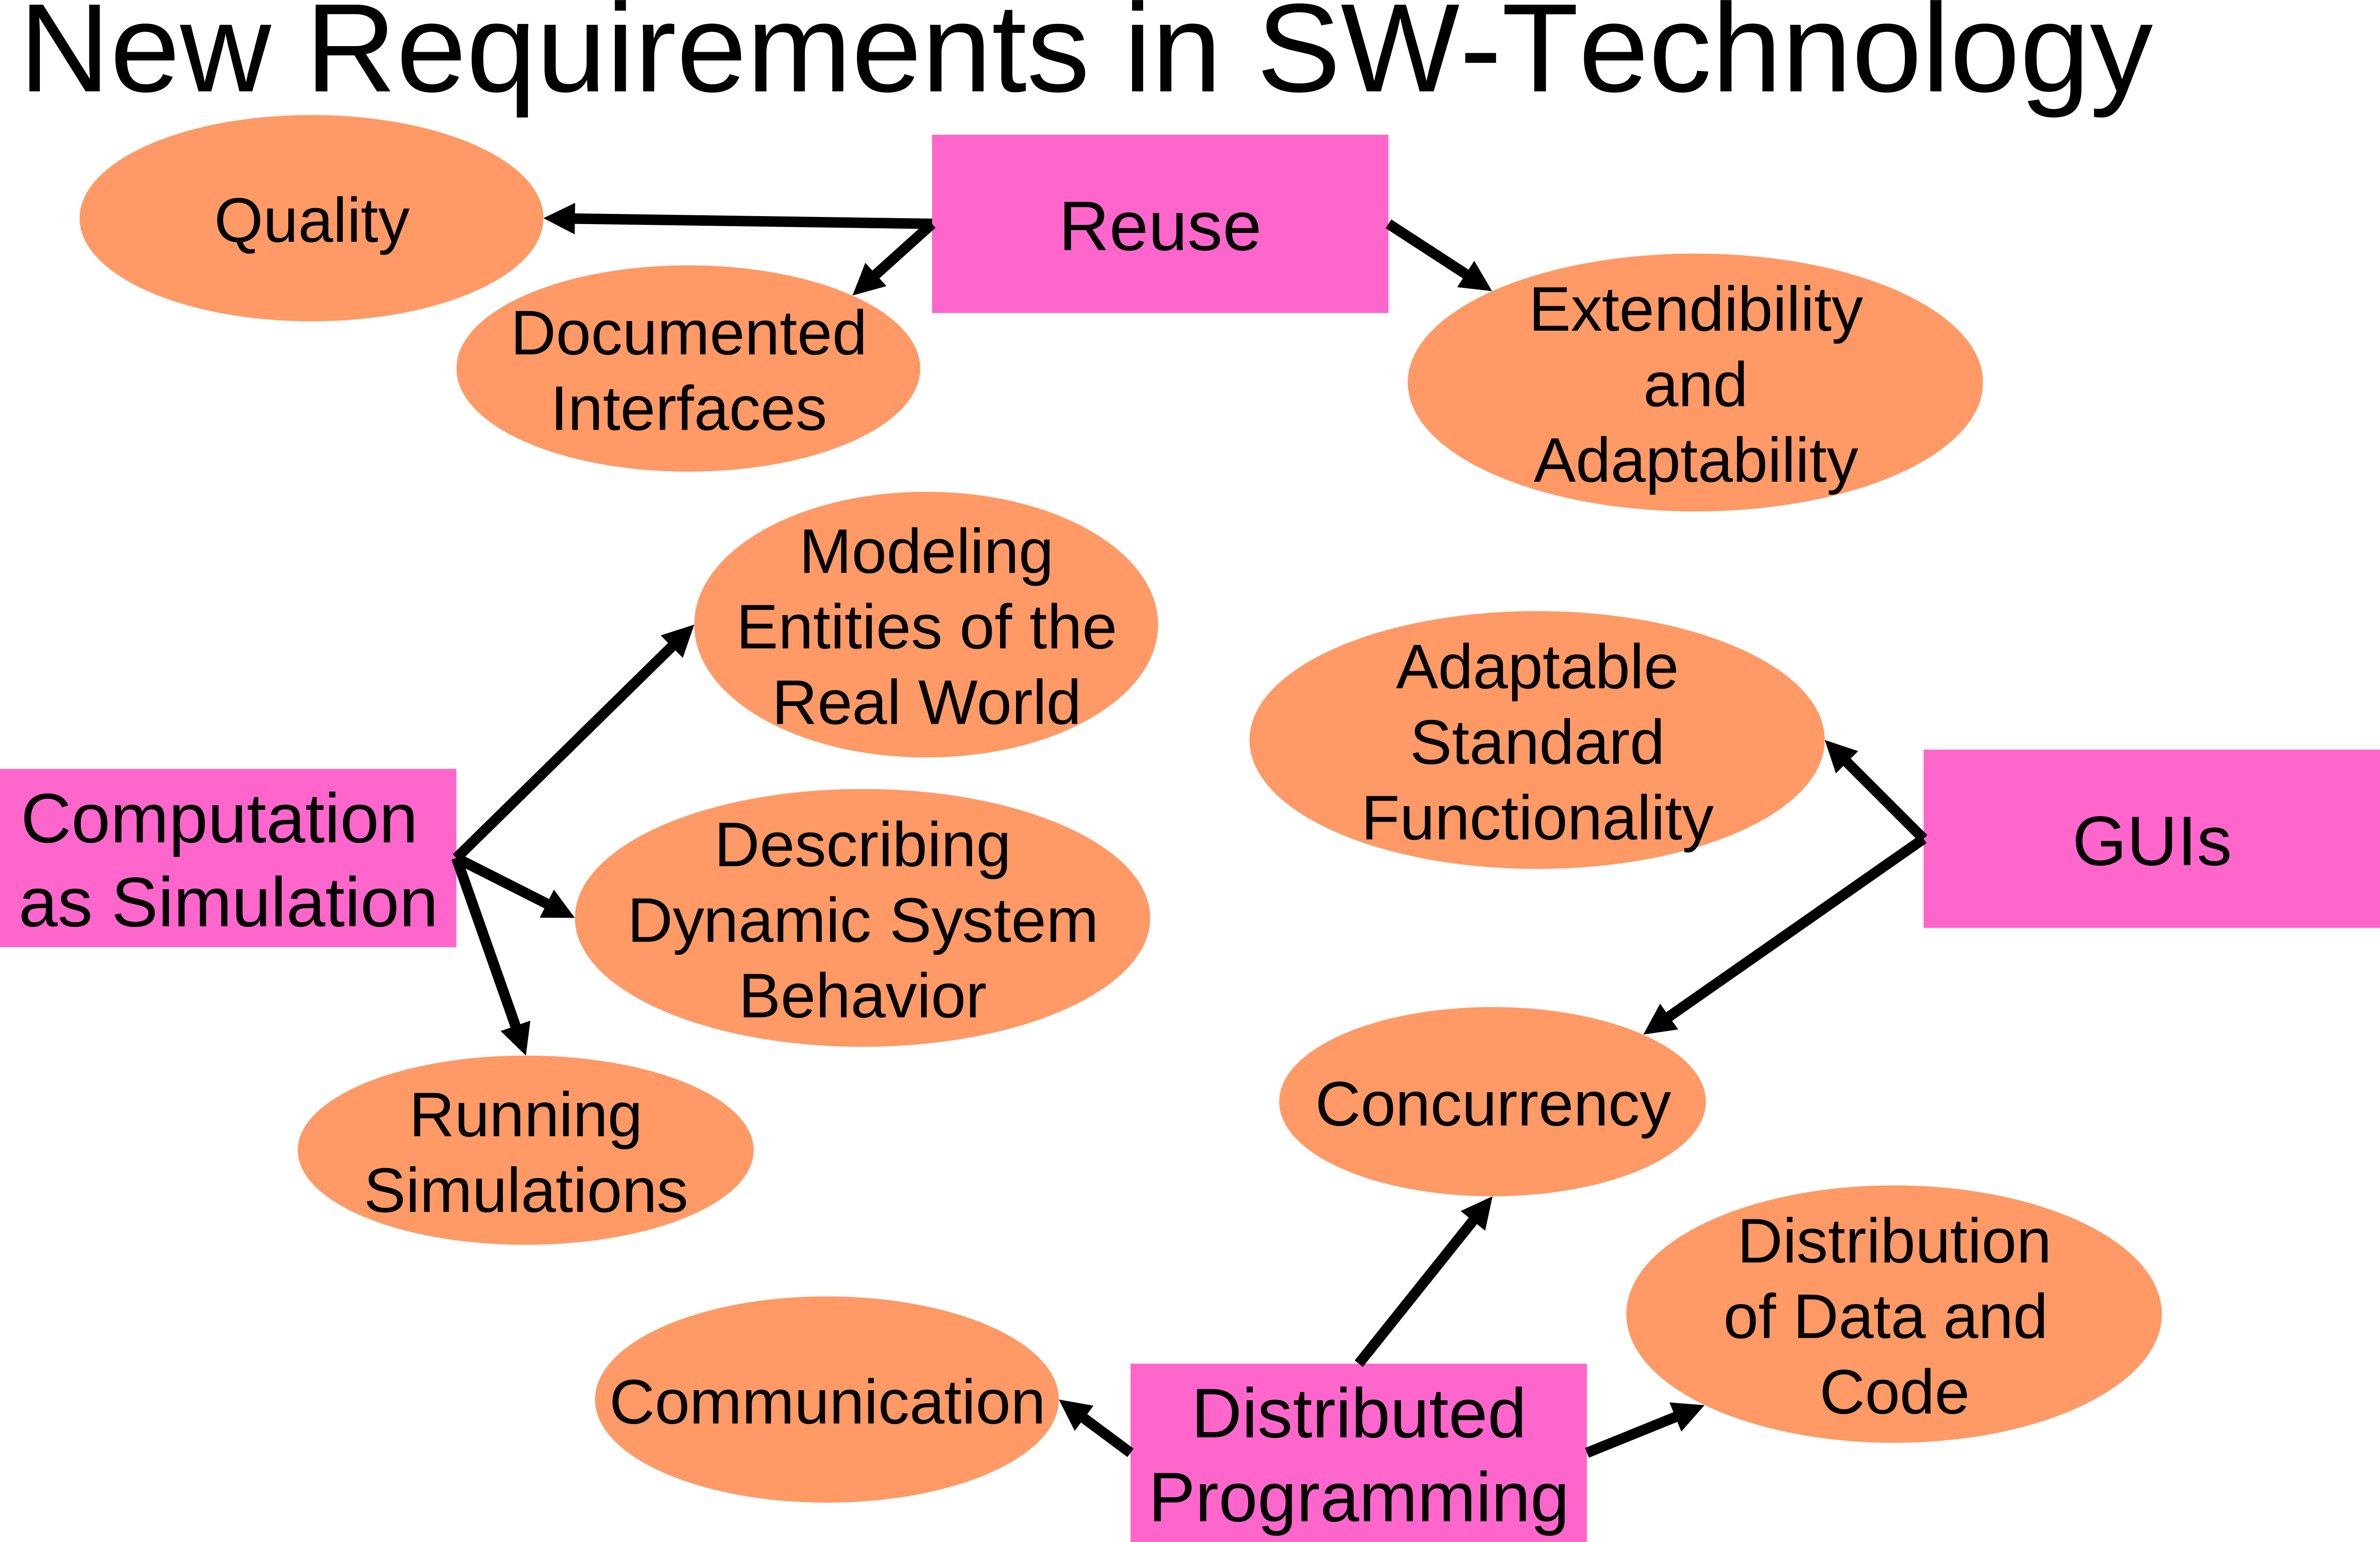
\includegraphics[width=0.7\textwidth]{img/01_new_requirements}
      \caption{New Requirements in Software Technology}
\end{figure}

\subsection{Study: Reusing Imperative Programs}
We try to model a University Administration System:
\begin{itemize}
 \item Which models students and professors
 \item Stores one record for each student and each professor in a repository
 \item A procedure printAll prints all records in the repository
\end{itemize}

\lstset{language=C}
\begin{lstlisting}[caption=Implementation in C]
typedef struct {
  char *name;
  char *room;
  char *institute;
} Professor;

typedef struct {
  char *name;
  int  regnum;
} Student;

void printStudent(Student *s) {...}
void printProf(Professor *p) {...}

typedef struct {
  enum { STU,PROF } kind;
  union {
    Student *s;
    Professor *p;
  } u;
} Person;

typedef Person **List;

void printAll( List l ) {
  int i;
  for ( i=0; l[ i ] != NULL; i++ )
    switch ( l[ i ] -> kind ) {
    case STU:
      printStudent( l[ i ] -> u.s );
      break;
    case PROF:
      printProf( l[ i ] -> u.p );
      break;
  }
}
\end{lstlisting}

\paragraph{Extending the System} in order to extend the system with assistants on has to:
\begin{itemize}
 \item Add a record and print function for the assistants
 \item Reuse old code for repository and printing
\end{itemize}

\begin{lstlisting}[caption=Extending the system]
// Student and Professor structs
typedef struct {
  char *name;
  char PhD_student; /* ‘y‘, ‘n‘ */
} Assistant;

// Student and Professor print code
void printAssi(Assistant *a) {...}

// Change the Person struct
typedef struct {
  enum { STU,PROF,ASSI } kind;
  union {
    Student *s;
    Professor *p;
    Assistant *a;
  } u;
} Person;

// Change the printAll function
void printAll( List l ) {
  int i;
  for ( i=0; l[ i ] != NULL; i++ )
    switch ( l[ i ] -> kind ) {
    case STU:
      printStudent( l[ i ] -> u.s );
      break;
    case PROF:
      printProf( l[ i ] -> u.p );
      break;
    case ASSI:
      printAssi( l[ i ] -> u.a );
      break;
  }
}
\end{lstlisting}

\subsection{Reuse in Imperative Languages}
\begin{itemize}
 \item Imperative languages don't have an explicit language support for extension and adaption
 \item Adaption usually requires modification reused code
 \item Code adaption requires \textbf{Copy-and-paste reuse} which leads to
  \begin{itemize}
   \item Code duplication
   \item Is difficult to maintain
   \item Is \emph{Error-prone}
  \end{itemize}

\end{itemize}

\subsection{Core Requirements}
All of this leads to these core requirements for object oriented programming languages:
\begin{figure}[h!]
  \centering
    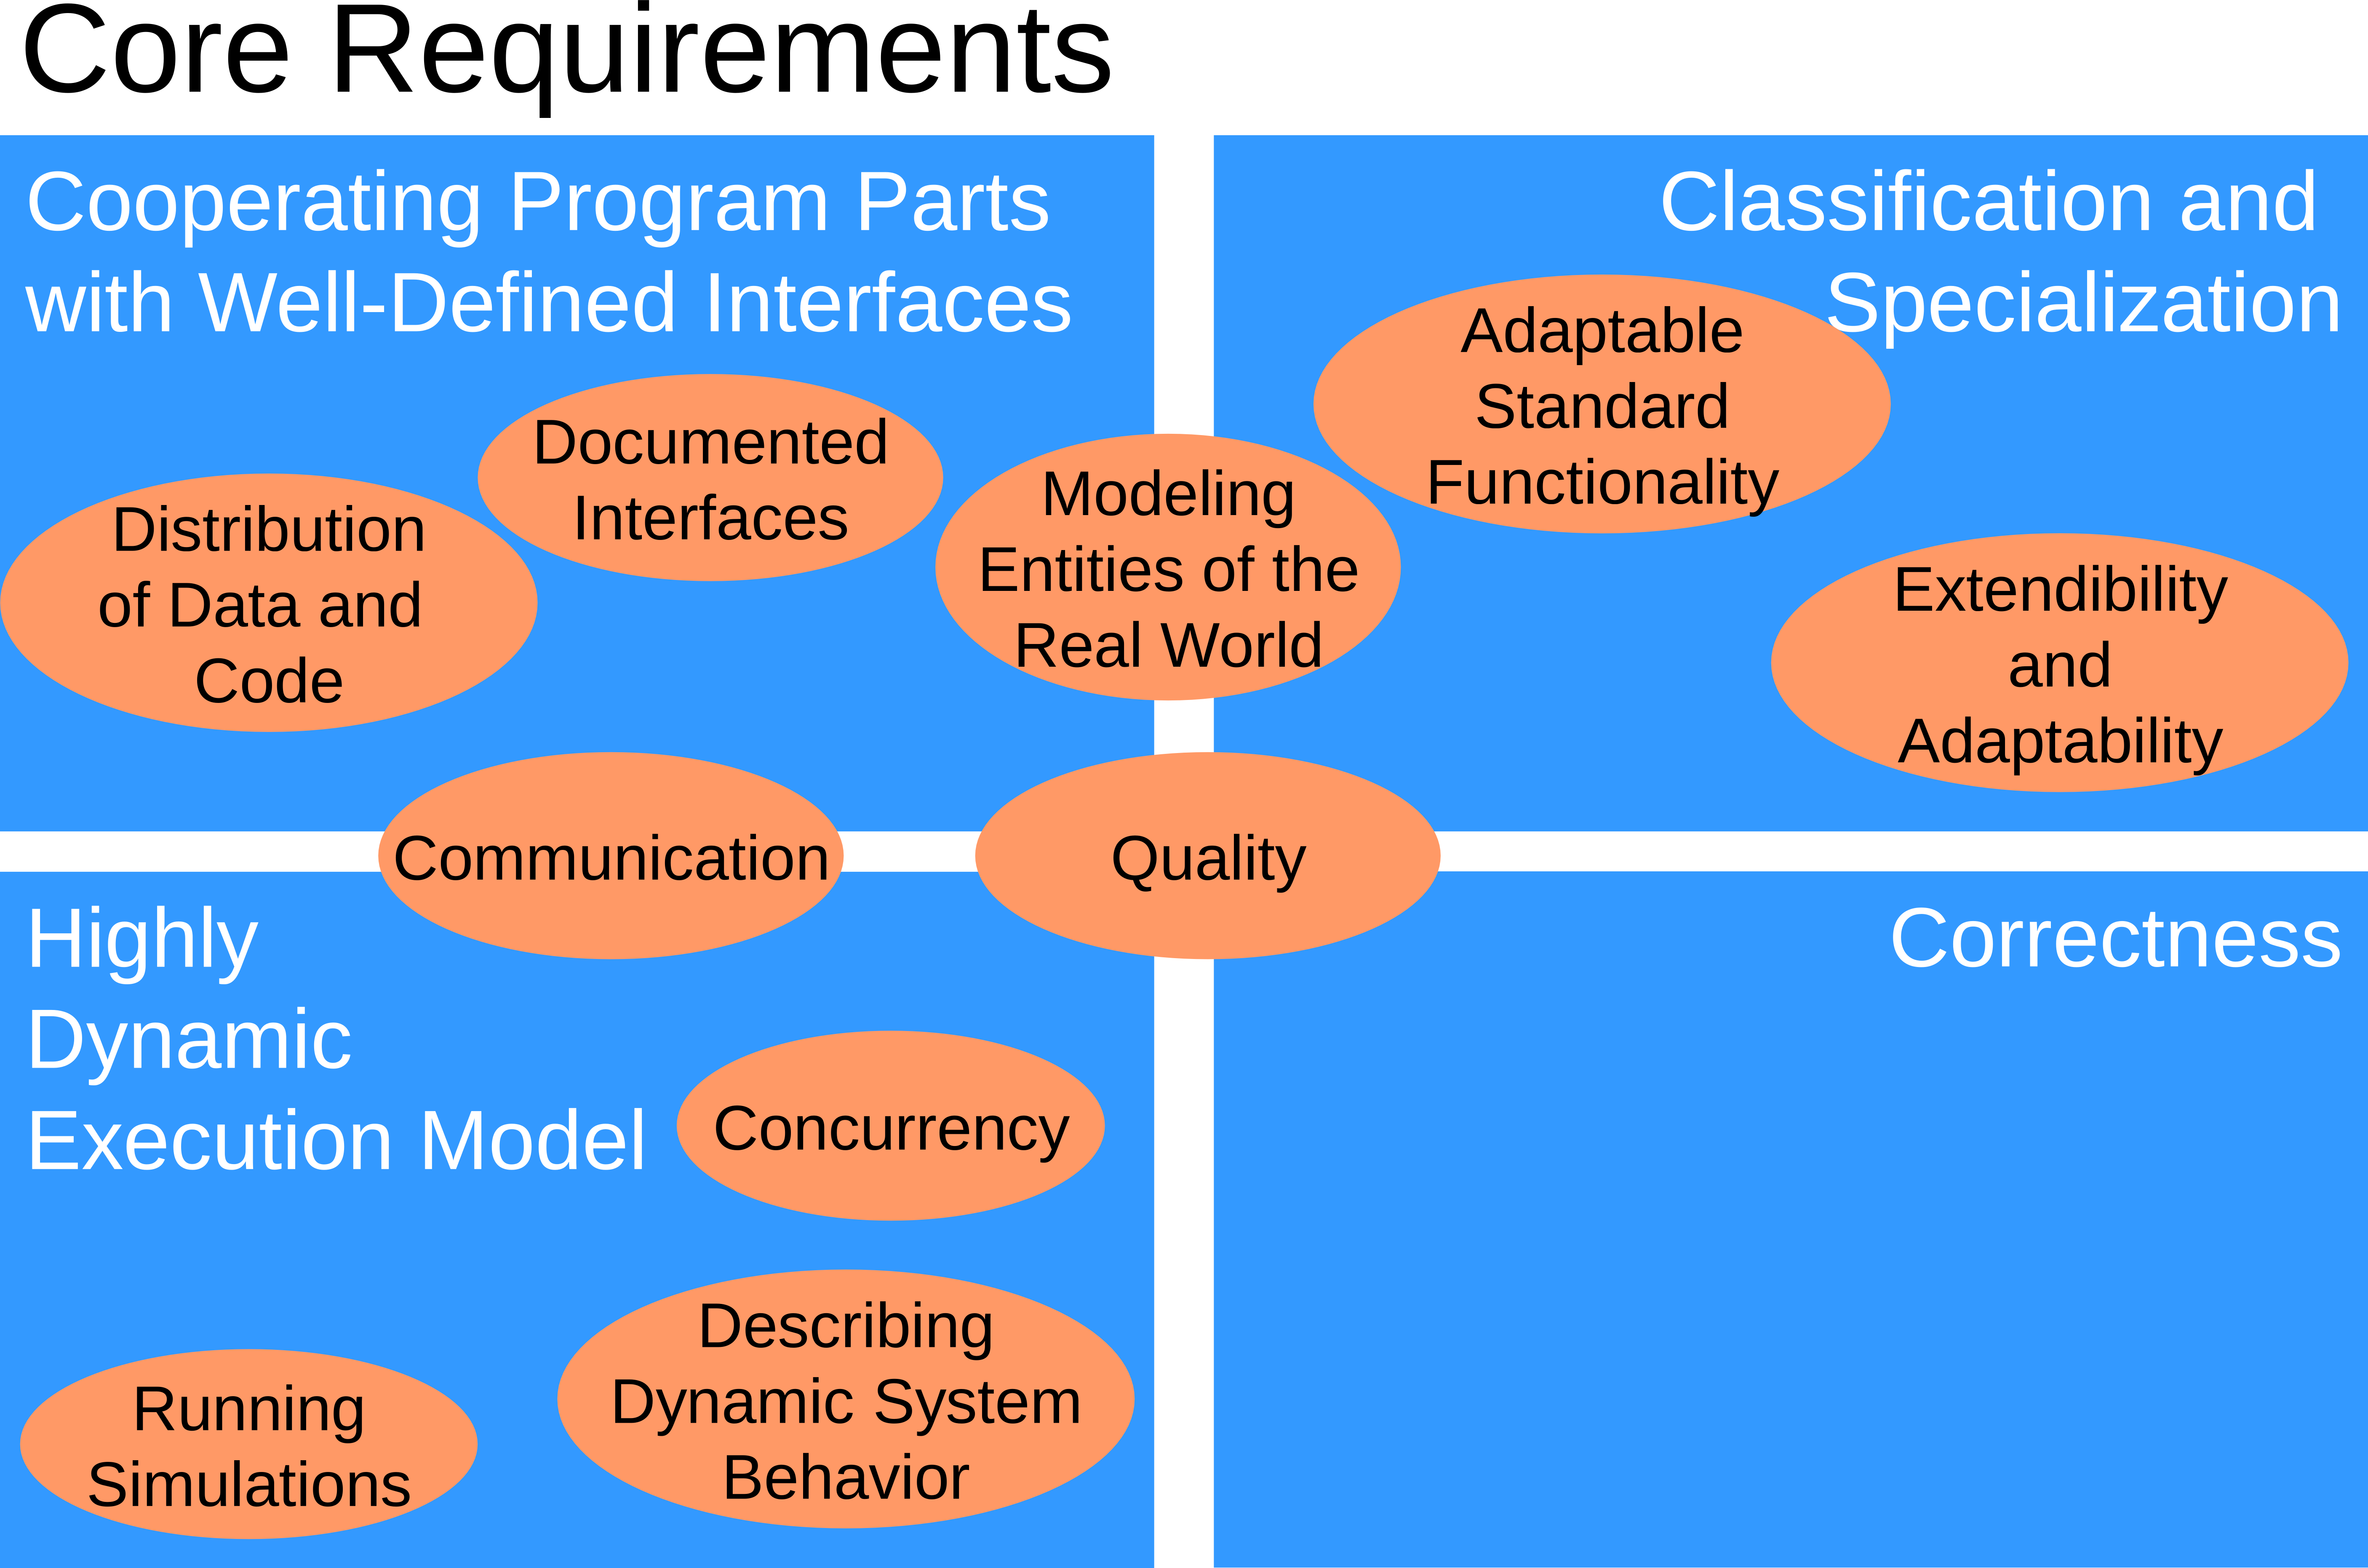
\includegraphics[width=0.7\textwidth]{img/01_core_requirements}
      \caption{Core Requirements in Software Technology}
\end{figure}

\section{Core Concepts}
\begin{shadequote}
The basic philosophy underlying object-oriented
programming is to make the programs as far as
possible reflect that part of the reality they are going
to treat. It is then often easier to understand and to
get an overview of what is described in programs.
The reason is that human beings from the outset are
used to and trained in the perception of what is going
on in the real world. The closer it is possible to use
this way of thinking in programming, the easier it is to
write and understand programs.\par\emph{Object-oriented Programming in the BETA Programming Language}
\end{shadequote}
\subsection{The Object Model}
\begin{itemize}
 \item A software system is a set of cooperating object
 \item Objects have state and processing ability
 \item Objects exchange messages
\end{itemize}
\begin{figure}[H]
  \centering
    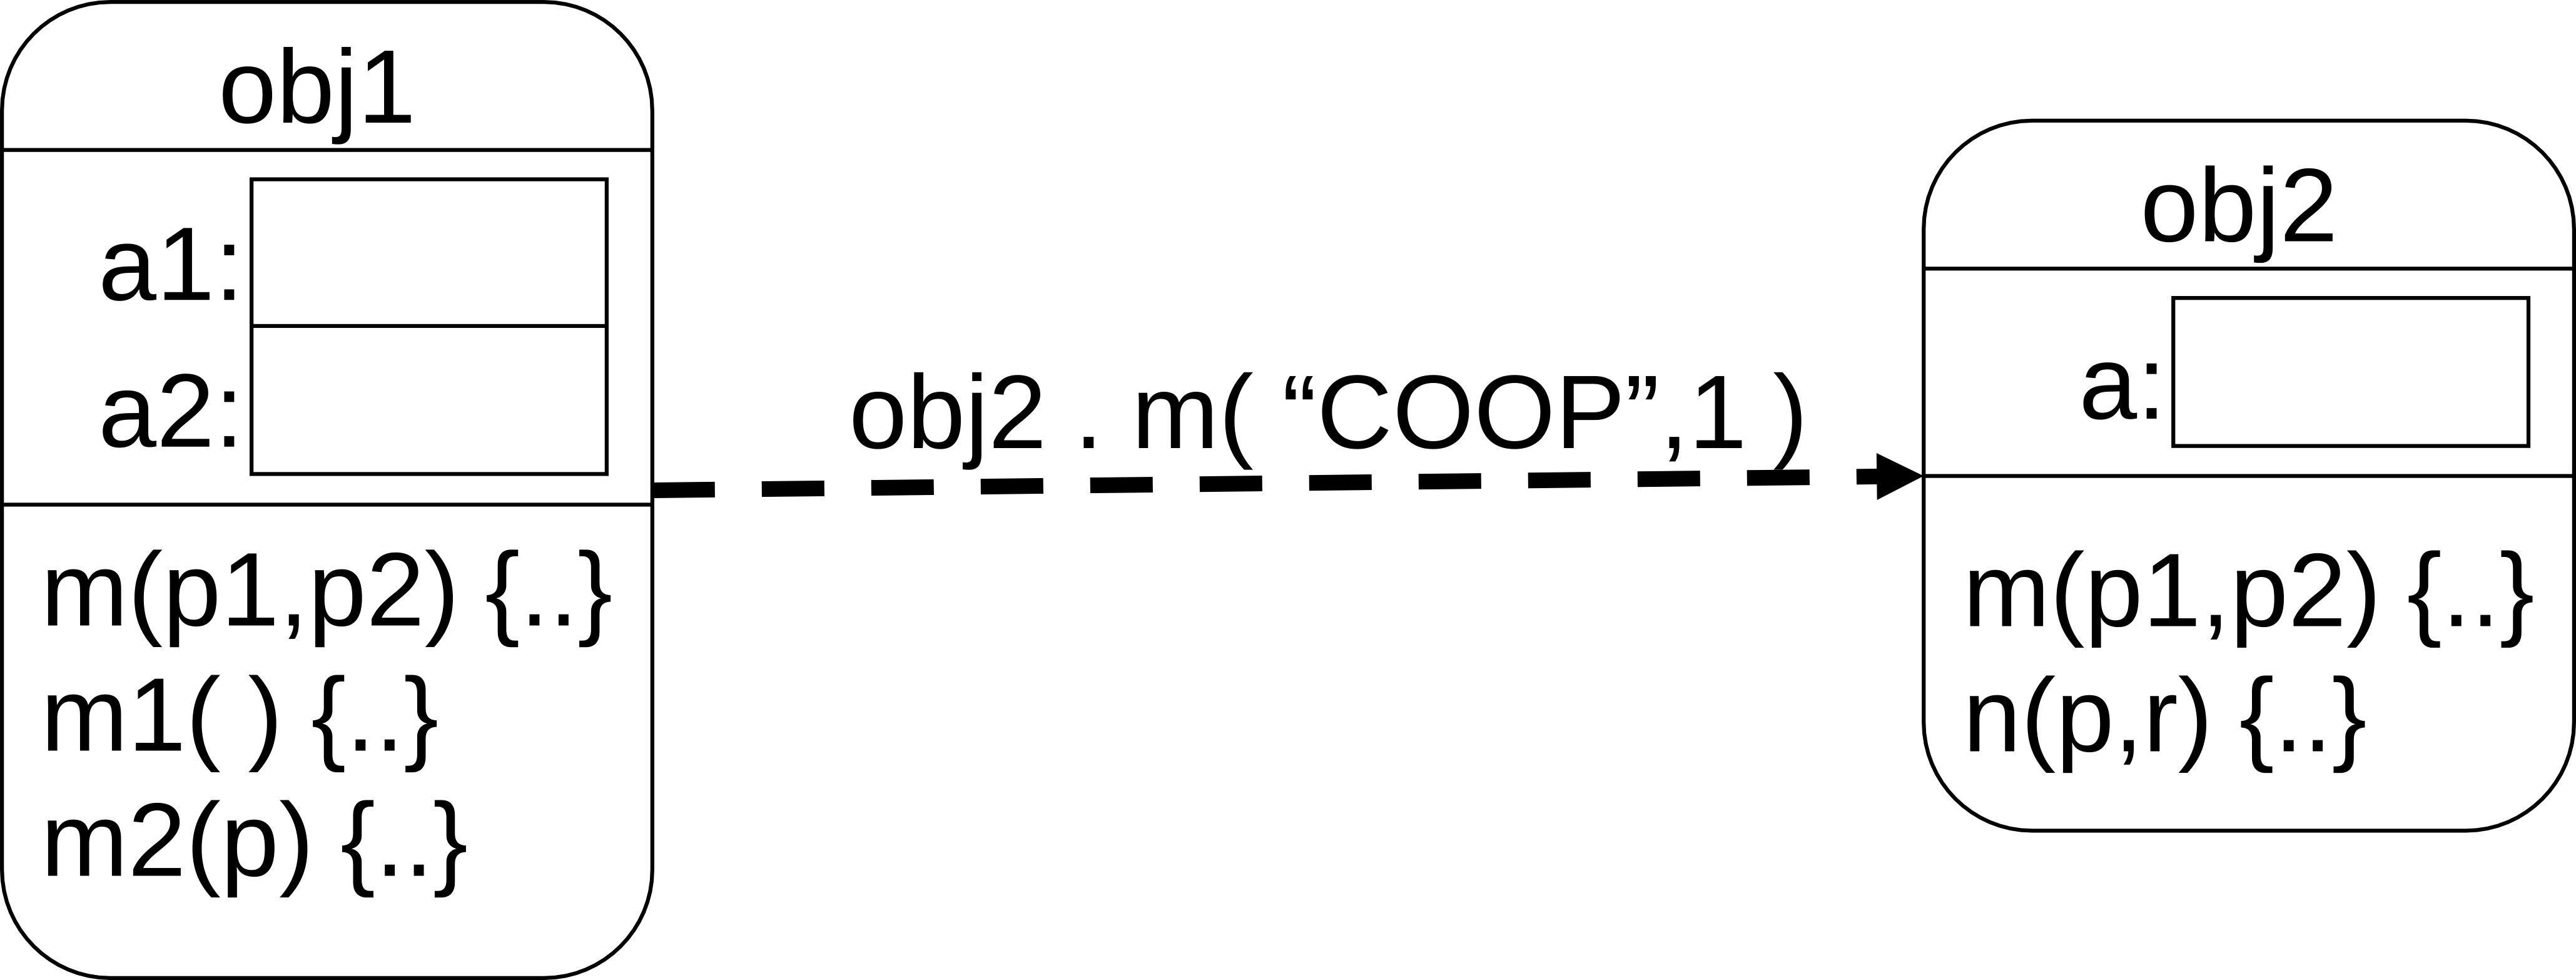
\includegraphics[width=0.5\textwidth]{img/01_object_model}
      \caption{The object model}
\end{figure}
\subsubsection{Characteristics of Objects}
\begin{itemize}
 \item State
 \item Identity
 \item Lifecycle
 \item Location
 \item Behavior
\end{itemize}
Compared to imperative programming, 
\begin{itemize}
 \item Objects lead to a \emph{different program structure}
 \item Objects lead to a \emph{different execution model}
\end{itemize}

\subsection{Interfaces and Encapsulation} 
\begin{itemize}
 \item Objects have \textbf{well-defined interfaces}
  \begin{itemize}
   \item Publicly accessible fields
   \item Publicly accessible methods
  \end{itemize}
 \item \text{Implementation is hidden} behind interface
  \begin{itemize}
   \item Encapsulation
   \item Information hiding
  \end{itemize}
 \item Interfaces are the basis for \textbf{describing behavior}
\end{itemize}

\subsection{Classification and Polymorphism}
\begin{itemize}
 \item \textbf{Classification}: Is a hierarchical structuring of objects
 \item Objects belong to different classes simultaneously
 \item \textbf{Substitution principle}: Subtype objects can be used wherever supertype objects are expected.
\end{itemize}

\begin{definition}[Classification]
Classifying is a general technique to hierarchically
structure knowledge about concepts, items, and
their properties.\\
The result is called classification.
\end{definition}

\paragraph{Characteristics of Classifications} We can classify objects or fields:
\begin{itemize}
 \item Classifications can be \emph{trees} or \emph{DAGs}
 \item Classifications of objects form \emph{``is-a'' relation}.
 \item Classes can be \emph{abstract} or \emph{concrete}.
\end{itemize}
\begin{definition}[Substitution principle]
Objects of subtypes can be used wherever objects are expected.
\end{definition}

\subsection{Polymorphism}
\begin{shadequote}
The quality of being able to assume different forms.\par\emph{Merriam-Webster Dictionary}
\end{shadequote}

\begin{definition}A program part is polymorphic if it can be used for objects of several types.
\end{definition}

\paragraph{Subtype Polymorphism} is a direct consequence of the substitution principle.
\begin{itemize}
 \item Program parts working with supertype objects work as well with subtype objects
 \item Example: \lstinline{ printAll } can print objects of class Person, Student, Professor, etc.
\end{itemize}
\subsection{Other forms of polymorphism}
\begin{description}
 \item[Parametric Polymorphism] Generic types
  \begin{itemize}
   \item Uses \emph{type parameters}
   \item One implementation can be used for different types
   \item \emph{Type mismatches can be detected at compile time}
  \end{itemize}
  \lstset{language=Java}
  \begin{lstlisting}
  class List<G> {
    G[ ] elems;
    void append( G p ) { ... }
  }
  
  List<String> myList;
  myList = new List<String>( );
  myList.append( “String” );
  \end{lstlisting}
 \item[Ad-hoc Polymorphism] Method overloading
  \begin{itemize}
   \item Allows several methods with the \emph{same name but different arguments}
   \item Also called \emph{overloading}
   \item No semantic concept: Can be modeled by \emph{renaming}
  \end{itemize}
  \begin{lstlisting}
  class Any {
    void foo( Polar p ) { ... }
    void foo( Coord c ) { ... }
  }
  x.foo( new Coord( 5, 10 ) );
  x.foo( new Polar( 5, 10 ) );
  \end{lstlisting}
\end{description}

\subsection{Specialization}
\begin{definition}
 Adding specific properties to an object or refining a concept by adding further characteristics.
\end{definition}




\end{document}
